

\begin{figure}
\begin{minipage}[height=.4\textheight]{.5\textwidth}
\centering \small{\texttt{(a)}}\\
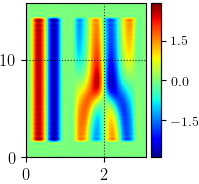
\includegraphics[width=.3\textwidth,height=.15\textheight]{MNG_01_initial}
\end{minipage}
\begin{minipage}[height=.4\textheight]{.5\textwidth}
\centering \small{\texttt{(b)}}\\
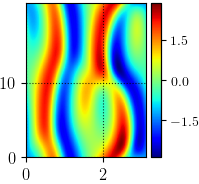
\includegraphics[width=.3\textwidth,height=.18\textheight]{MNG_01_final}
\end{minipage}
\caption{ \label{fig:block01}
(a) Initial \spt\ field for the one-by-two symbolic block given by \refeq{e-block01}
(b) \twoT\ resultant from numerically converging (a),
$[\speriod{b},\period{b}]=[3.13\cdots,20.84\cdots]$
}
\end{figure}

\begin{figure}
\begin{minipage}[height=.4\textheight]{.5\textwidth}
\centering \small{\texttt{(a)}}\\
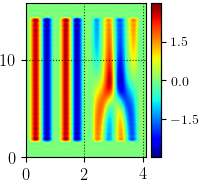
\includegraphics[width=.4\textwidth,height=.15\textheight]{MNG_001_initial}
\end{minipage}
\begin{minipage}[height=.4\textheight]{.5\textwidth}
\centering \small{\texttt{(b)}}\\
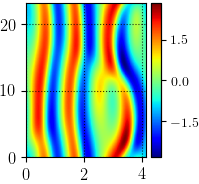
\includegraphics[width=.4\textwidth,height=.23\textheight]{MNG_001_final}
\end{minipage}
\caption{ \label{fig:block001}
(a) Initial \spt\ field for the one-by-three symbolic block given by \refeq{e-block001}
(b) \twoT\ resultant from numerically converging (a),
$[\speriod{b},\period{b}]=[4.12\cdots,23.15\cdots ]$.
}
\end{figure}




% Example that shows transformation of gap to merger
\begin{figure}
\begin{minipage}[height=.4\textheight]{.5\textwidth}
\centering \small{\texttt{(a)}}\\
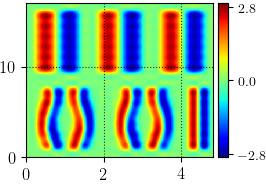
\includegraphics[width=.4\textwidth,height=.15\textheight]{MNG_000_220_initial}
\end{minipage}
\begin{minipage}[height=.4\textheight]{.5\textwidth}
\centering \small{\texttt{(b)}}\\
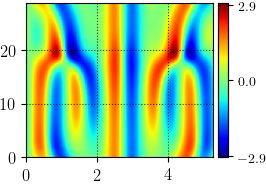
\includegraphics[width=.4\textwidth,height=.23\textheight]{MNG_000_220_final}
\end{minipage}
\caption{ \label{fig:block001}
(a) Initial \spt\ field for the one-by-three symbolic block given by \refeq{e-block001}
(b) \twoT\ resultant from numerically converging (a),
$[\speriod{b},\period{b}]=[4.12\cdots,23.15\cdots ]$.
}
\end{figure}

\begin{figure}
\begin{minipage}[height=.4\textheight]{.5\textwidth}
\centering \small{\texttt{(a)}}\\
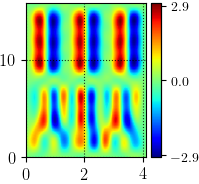
\includegraphics[width=.4\textwidth,height=.15\textheight]{MNG_000_101_initial}
\end{minipage}
\begin{minipage}[height=.4\textheight]{.5\textwidth}
\centering \small{\texttt{(b)}}\\
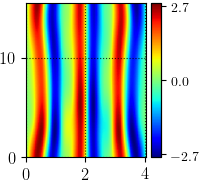
\includegraphics[width=.4\textwidth,height=.23\textheight]{MNG_000_101_final}
\end{minipage}
\caption{ \label{fig:block000_101}
(a) Initial \spt\ field for the one-by-three symbolic block given by \refeq{e-block001}
(b) \twoT\ resultant from numerically converging (a),
$[\speriod{b},\period{b}]=[4.12\cdots,23.15\cdots ]$.
}
\end{figure}

By looking at the set of converged gluings it lacks the pattern corresponding
to a gap being adjacent to a merger, spatially.
Indeed, in almost every

Here are some examples,

% Example of finding something too symmetric/shows conservation of wavenumber
%\begin{figure}
%\begin{minipage}[height=.4\textheight]{.5\textwidth}
%\centering \small{\texttt{(a)}}\\
%\includegraphics[width=.4\textwidth,height=.15\textheight]{MNG_22_11_initial}
%\end{minipage}
%\begin{minipage}[height=.4\textheight]{.5\textwidth}
%\centering \small{\texttt{(b)}}\\
%\includegraphics[width=.4\textwidth,height=.23\textheight]{MNG_22_11_final}
%\end{minipage}
%\caption{ \label{fig:block001}
%(a) Initial \spt\ field for the one-by-three symbolic block given by \refeq{e-block001}
%(b) \twoT\ resultant from numerically converging (a),
%$[\speriod{b},\period{b}]=[4.12\cdots,23.15\cdots ]$.
%}
%\end{figure}

\begin{figure}
\begin{minipage}[height=.4\textheight]{.5\textwidth}
\centering \small{\texttt{(a)}}\\
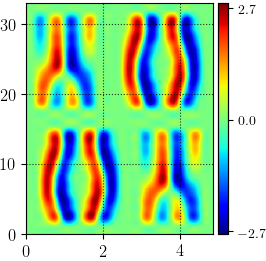
\includegraphics[width=.4\textwidth,height=.15\textheight]{MNG_12_21_initial}
\end{minipage}
\begin{minipage}[height=.4\textheight]{.5\textwidth}
\centering \small{\texttt{(b)}}\\
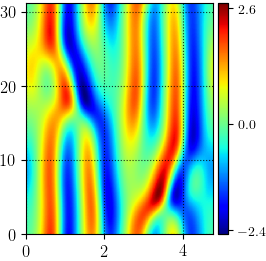
\includegraphics[width=.4\textwidth,height=.23\textheight]{MNG_12_21_final}
\end{minipage}
\caption{ \label{fig:block12_21}
(a) Initial \spt\ field for the one-by-three symbolic block given by \refeq{e-block001}
(b) \twoT\ resultant from numerically converging (a),
$[\speriod{b},\period{b}]=[4.12\cdots,23.15\cdots ]$.
}
\end{figure}

This process depends on the neighbors of the tiles as well; it seems to be primarily
influenced by spatial neighbors. For instance, in

%\begin{figure}
%\begin{minipage}[height=.4\textheight]{.5\textwidth}
%\centering \small{\texttt{(a)}}\\
%\includegraphics[width=.4\textwidth,height=.15\textheight]{MNG_002_210_initial}
%\end{minipage}
%\begin{minipage}[height=.4\textheight]{.5\textwidth}
%\centering \small{\texttt{(b)}}\\
%\includegraphics[width=.4\textwidth,height=.23\textheight]{MNG_002_210_final}
%\end{minipage}
%\caption{ \label{fig:block002_210}
%(a) Initial \spt\ field for the one-by-three symbolic block given by \refeq{e-block001}
%(b) \twoT\ resultant from numerically converging (a),
%$[\speriod{b},\period{b}]=[4.12\cdots,23.15\cdots ]$.
%}
%\end{figure}

\begin{figure}
\begin{minipage}[height=.05\textheight]{.5\textwidth}
\centering
\small{\texttt{(a)}} \\
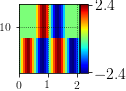
\includegraphics[width=.8\textwidth,height=.2\textheight]{MNG_streak_merger_initial}
\end{minipage}
\begin{minipage}[height=.2\textheight]{.5\textwidth}
\centering
\small{\texttt{(b)}} \\
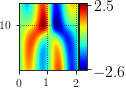
\includegraphics[width=.8\textwidth,height=.3\textheight]{MNG_streak_merger}
\end{minipage}
\caption{ \label{fig:streakmerger}
(a) Initial condition composed of three streaks and an region of zeros,
imbued on a {\spt} domain approximating the known tile's domain size.
(b) The tile that (a) converges to.
}
\end{figure}

